\section{Model}
\label{sec:model}

\subsection{Summary}

To alleviate these problems we propose a different model structure. Our model inherits many features from agent-based simulation models but replaces the contacts between moving particles by contacts between individuals who work, go to school, live in a household and enjoy leisure activities. The structure of the model is depicted in Figure~\ref{fig:model_graph}.

\begin{figure}[!ht]
    \centering
    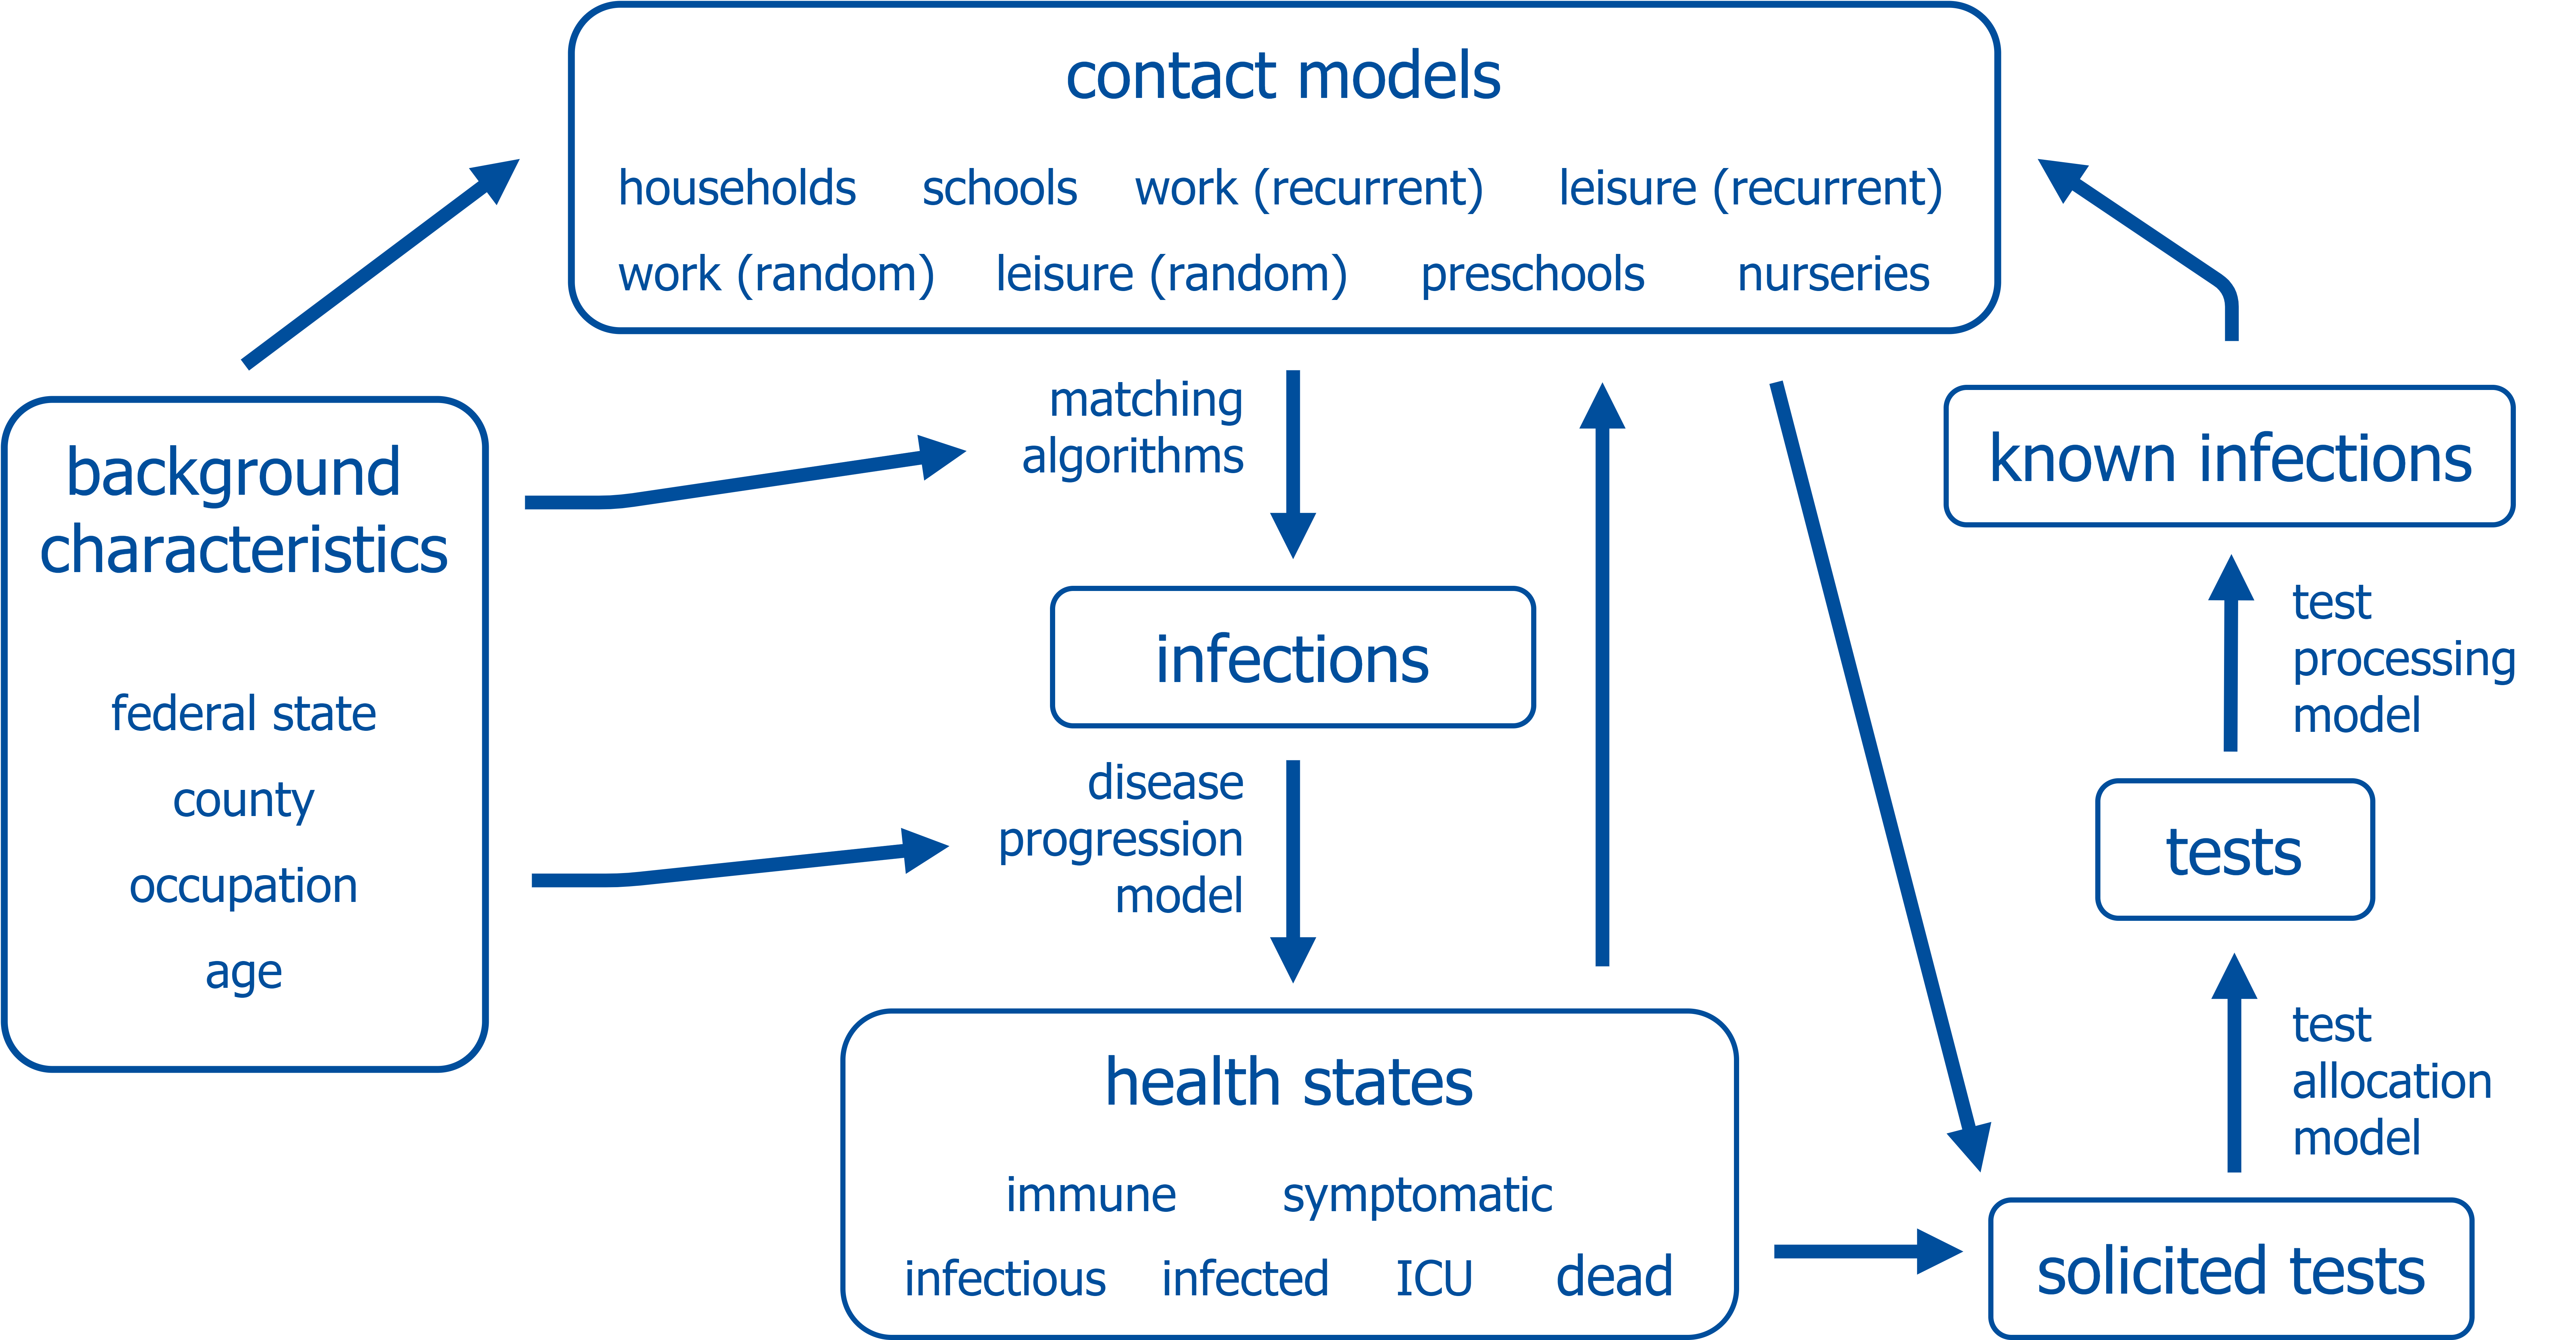
\includegraphics[width=0.7\textwidth]{../figures/model_detailed.png}
    \caption{Simplified graph of the model}
    \label{fig:model_graph}
\end{figure}

The background characteristics include age, county and occupation of each simulated individual. Contact models are functions that map individual characteristics into a predicted number of contacts. Currently we distinguish between eight types of contact models which are all listed in Figure \ref{fig:model_graph}: households, recurrent and random work contacts, recurrent and random leisure contacts, and nursery, preschool, and school contacts.

The predicted number of contacts is translated into infections by a matching algorithm. There are different matching algorithms for recurrent contacts (e.g. classmates, family members) and non-recurrent contacts (e.g. clients, contacts in supermarkets). The infection probability can differ for each contact type. All types of contacts can be assortative with respect to geographic and demographic characteristics.

Once a person is infected, the disease progresses in a fairly standard way which is also depicted in Figure~\ref{fig:course_of_disease}. Asymptomatic cases and cases with mild symptoms are infectious for some time and recover eventually. Cases with severe symptoms additionally require hospitalization and lead to either recovery or death.

People who experience symptoms as well as people who had a risk contact can demand a test. Test allocation models that take into account the testing capacity determine which individuals actually receive a test. Test processing models determine in which order the tests are processed and when infected individuals are notified.

In addition, people who have symptoms, received a positive test, or had a risk contact can reduce their number of contacts across all contact types endogenously.

The model makes it very simple to translate policies into model quantities. For example, school closures imply the complete suspension of school contacts. A strict lockdown implies shutting down work contacts of all people who are not employed in a systemically relevant sector. It is also possible to have more sophisticated policies that condition the number of contacts on observable characteristics, risk contacts or health states.

Another key advantage of the model is that the number of contacts an individual has of each contact type can be calibrated from publicly available data \citep{Mossong2008}. This in turn allows us to estimate policy-invariant infection probabilities from time series of infection and death rates using the method of simulated moments \citep{McFadden1989}. Since the infection probabilities are time-invariant, data collected since the beginning of the pandemic can be used for estimation. Moreover, since we can model the testing strategies that were in place at each point in time, we can correct the estimates for the fact that not all infections are observed.

In the following sections we describe each of the model components in more detail.

\subsection{Modeling Numbers of Contacts}
\label{sec:number_of_contacts}

Consider a hypothetical population of 1,000 individuals in which 50 were infected with a novel infectious disease. From this data alone, it is impossible to say whether only those 50 people had contact with an infectious person and the disease has an infection probability of 1 in each contact or whether everyone met an infectious person but the disease has an infection probability of only 5 percent per contact. SEIR models do not even try to distinguish contact frequency from the infectiousness of each contact and combine the two in one parameter that is not invariant to social distancing policies.

To model social distancing policies, we need to disentangle the effects of the number of contacts of each individual and the effect of policy-invariant infection probabilities specific to each contact type. Since not all contacts are equally infectious, we distinguish different contact types.

The number and type of contacts in our model can be easily extended. Each type of contacts is described by a function that maps individual characteristics, health states and the date into a number of planned contacts for each individual. This allows to model a wide range of contact types.

Currently, there are the following contact types:

\begin{itemize}
    \item Households: Each household member meets all other household members every day. The household sizes and structures are calibrated to be representative for Germany.
    \item Random non-work contacts: Each person has contacts with randomly drawn other people. This contact type reflects contacts during pure leisure activities as well as non leisure activities such as grocery shopping or medical appointments.
    \item Random work contacts: Each working adult has contact to randomly drawn other people.
    \item Recurrent daily work contacts: Each working adult meets other workers every day. This is meant to capture work colleagues.
    \item Recurrent weekly work contacts: Each working adult meets other workers once per week. We randomize over the days on which the meetings take place. This is meant to capture meetings with clients, superiors or other colleagues which happen infrequently.
    \item Schools: Each student meets all of his classmates every day. Class sizes are calibrated to be representative for Germany. Schools are closed on weekends and during vacations, which vary by states.
    \item Preschools: Similar to schools but for younger children.
    \item Nurseries: Similar to schools but for very young children.
\end{itemize}


The number of random and recurrent contacts at the workplace and at home is calibrated with data provided by \cite{Mossong2008}. For details see Section~\ref{sec:calibration}. In particular, we sample the number of contacts or group sizes from empirical distributions that sometimes depend on age. Instead it would also be possible to use economic or other behavioral models to predict the number of contacts.

Theoretically, each contact type can have its own infection probability. However, to reduce the number of free parameters and thus avoid a potential over-fitting we impose some constraints. For now, infection probabilities in schools, preschools and nurseries are equal. Moreover, we restrict all work contacts to have the same infection probability.


\subsection{Reducing Numbers of Contacts Through Policies}
\label{sec:policies}

The main motivation of our model is to predict the effect of policies that affect the number of contacts people have. Examples range from school closures and lockdowns to more nuanced policies such as a mandatory quarantines for symptomatic individuals or a class splitting policy where only half of the students come to school in person and the other half joins digitally with weekly rotation.

Instead of thinking of policies as completely replacing how many contacts people have, it is often more helpful to think of them as adjusting the pre-pandemic number of contacts.

Therefore, we implement policies as a step that happens after the number of contacts is calculated but before individuals are matched.

On an abstract level, a policy is a functions that modifies the number of contacts of one contact type. For example, school closures simply set all school contacts to zero. A lockdown where only essential workers are allowed to work means that approximately two thirds of the working population have zero work contacts and the rest has the same number of contacts as before.

% importance of fine-grained contact types and having the entire population
This, in conjunction with our fine grained contact types, allows us to easily implement a wide variety of policies. Allowing policies to depend on the health states of the entire population means that adaptive lockdowns where, for example, schools close when a certain threshold of infections is surpassed at the county level would be as simple as determining which counties are above the threshold and then setting all school contacts in these counties to zero.

The dependency of policies on health states also makes it possible to model contact tracing. For example, a policy could check whether each child has a classmate who's received a positive test result and then bar all children of that class from attending school.

% contact tracing and how including the states means the sky is the limit
Some policies can be easily implemented if the background characteristics are suitably extended. For example, a schooling policy with split classes, where each half attends school every other week can be implemented by storing whether the child would attend in even or odd weeks in the background characteristics and then using that information in the policy function.

For some policies the exact effect on each contact type is not easy to determine. If this refers to a policy during the estimation period, it is possible to estimate such parameters by fitting the model to time series data of infection rates. This is only possible if the policy was not active during the whole estimation period and thus the infection probabilities can be identified separately. If instead it refers to a policy that we want to simulate, we make a scenario analysis in which the model is simulated with several assumptions about how the policy affects the number of contacts.


\subsection{Endogenous Contact Reductions}
\label{sec:endogenous_contact_reductions}

Policies are not the only way in which the number of contacts are reduced compared to the pre-pandemic level. It is important to model those other channels. Otherwise, the effect of policies would be overestimated and policy recommendations based on the model would be biased.

Examples of endogenous contact reductions are manifold: symptomatic people stay at home; Members of risk groups try to reduce their number of contacts more strongly than others; People self-isolate if they know they had a risk contact.

Since we model the number of contacts as arbitrary functions of background characteristics and health states, it is easy to implement such considerations.

In our current empirical application we only model that symptomatic people reduce their number of contacts across all contact types (except for households) by 70 \%. Within households they reduce contacts by 50\%. We are working on extending this to allow for formal and informal contact tracing as well as quarantines after positive test results.


\subsection{Matching Individuals}
\label{sec:matching}

The empirical data described above only allows to estimate the number of contacts each person has. In order to simulate transmissions of Covid-19, the numbers of contacts has to be translated into actual meetings between people. This is achieved by matching algorithms:

As described in section \ref{sec:number_of_contacts}, some contact types are recurrent (i.e. the same people meet regularly), others are non-recurrent (i.e. it would only be by accident that two people meet twice). The matching process is different for recurrent and non recurrent contact models.

Recurrent contacts are described by two components: 1) A variable in the background characteristics. An example would be a school class identifier which could come from actual data or be drawn randomly to achieve representative class sizes. 2) A deterministic or random function that takes the value 0 (non-participating) and 1 (participating) and can depend on the weekday, date and health state. This can be used to model vacations, weekends or symptomatic people who stay home (see section \ref{sec:endogenous_contact_reductions} for details).

The matching process for recurrent contacts is then extremely simple: On each simulated day, every person who does not stay home meets all other group members who do not stay home. The assumption that all group members have contacts with all other group members is not fully realistic, but seems like a good approximation to reality, especially in light of the suspected role of aerosol transmission for Covid-19 (\cite{Morawska2020, Anderson2020}).

The matching in non-recurrent contact models is more difficult and implemented in a two stage sampling procedure to allow for assortative matching. Currently most contact models are assortative with respect to age (it is more likely to meet people from the same age group) and county (it is more likely to meet people from the same county) but in principle any set of discrete variables can be used. This set of variables that influence matching probabilities introduce a discrete partition of the population into groups. The first stage of the two stage sampling process samples on the group level. The second stage on the individual level.

Below, we first show pseudo code for the non-recurrent matching algorithm and then describe how the algorithm works in words.

%%% ToDo: Get syntax highlighting for the pseudo code. Try out different languages.

\begin{lstlisting}
while unmatched contacts remain:
    model, id = draw contact model and individual
    for contact in remaining_contacts[id, model]:
        draw group of other person
        draw other person from that group
        determine if id infects other or vice versa
        remaining_contacts[id, model] -= 1
        remaining_contacts[other, model] -= 1
\end{lstlisting}


We first randomly draw a contact type and individual. For each contact oth the drawn contact type that person has, we first draw the group of the other person (first stage). Next, we calculate the probability to be drawn for each member of the group, based on the number of remaining contacts. I.e. people who have more remaining contacts are drawn with a higher probability. This has to be re-calculated each time because with each matched contact, the number of remaining contacts changes. We then draw the other individual, determine whether an infection takes place and if so update the health states of the newly infected person. Finally, we reduce the number of remaining contacts of the two matched individuals by one.

The recalculation of matching probabilities in the second stage is computationally intensive because it requires summing up all remaining contacts in that group. Using a two stage sampling process where the first stage probabilities remain constant over time makes the matching computationally much more tractable because the number of computations increases quadratically in the second stage group size.

\FloatBarrier


\subsection{Course of the Disease}

The following medical parameters describing the progression of the disease are taken from systematic reviews (e.g. \cite{He2020}). After an infection occurs, the disease progresses in the way depicted in Figure~\ref{fig:course_of_disease}.

\begin{figure}[!ht]
    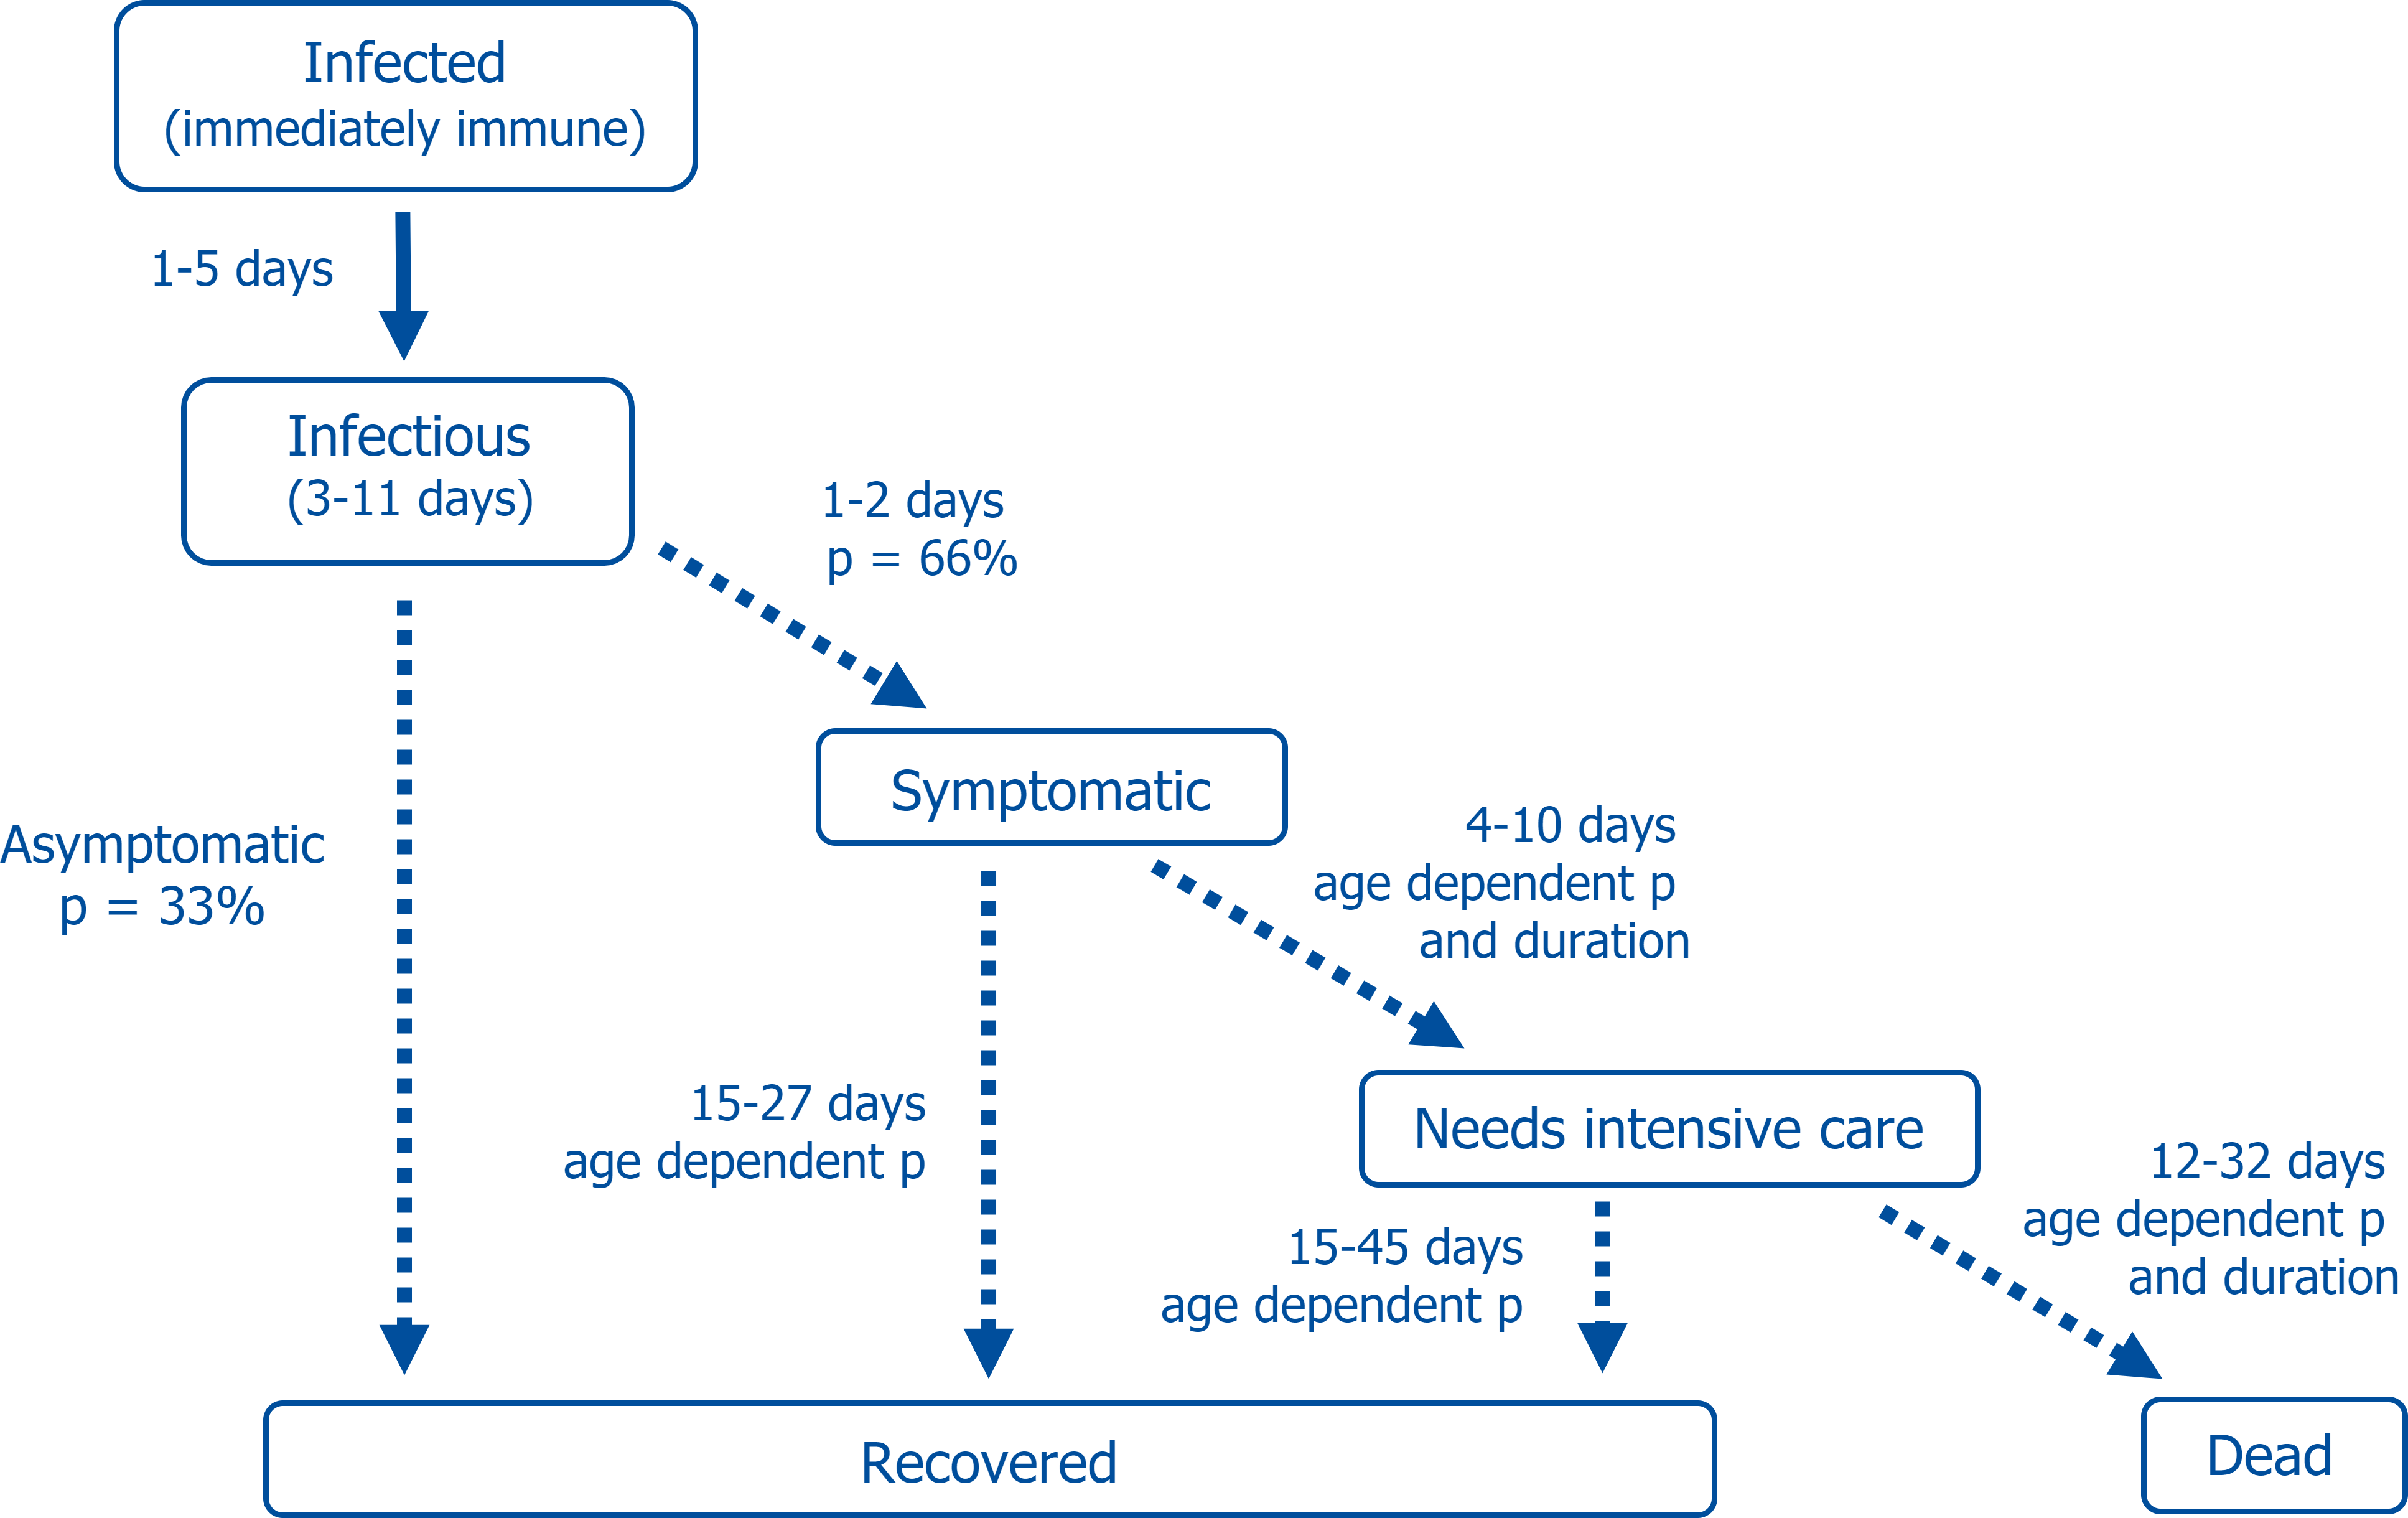
\includegraphics[width=0.7\textwidth]{../figures/disease_progression.png}
    \caption{Course of Disease in the model}
    \label{fig:course_of_disease}
\end{figure}

First, infected individuals will become infectious after one to five days. About one third of people stays asymptomatic. The rest develops symptoms about one to two days after they become infectious. Modeling asymptomatic and pre-symptomatic cases is important because those people do not reduce their contacts or demand a test and can potentially infect many other people \citep{Donsimoni2020}.

A small share of symptomatic people will develop strong symptoms that require intensive care. The exact share and time span is age-dependent. An age-dependent share of intensive care unit (ICU) patients will die after spending up to 32 days in intensive care. Moreover, if the ICU capacity was reached, all patients who require intensive care but do not receive it die.

It would be easy to make the course of disease even more fine grained. For example, we could model people who require hospitalization but not intensive care. So far we opted against that because only the ICU capacity might become a bottleneck in Germany.

We allow the progression of the disease to be stochastic in two ways: Firstly, state changes only occur with a certain probability (e.g. only a fraction of infected individuals develops symptoms). Secondly, the number of periods for which an individual remains in a state is drawn randomly. The parameters that govern these processes are taken from the literature. They can vary with the age of an individual.

Detailed information on the calibration of the disease parameters is available as part of our \href{https://sid-dev.readthedocs.io/en/latest/reference_guides/epi_params.html}{online documentation}.
